\section{A conceptual frame for building Process-Aware Model-Driven Development
environments}
\label{sec:meta}

\subsection{A Generic Requirements Gathering Framework}
\label{sec:generic_req_fram}

The case study requirements gathering framework we introduce here borrows its
structure from the Model-based Integrated Requirement Specification and Analysis (MIRA)
Framework~\cite{MIRA13}. The main parts of the MIRA framework are
as follows:
\begin{itemize}
  \item The \emph{system context} describes the relevant elements that belong
  to the context of the system being developed.
  \item The \emph{requirement list} documents the capabilities and limitations
  of the system under development.
  \item The \emph{trace link list} keeps the relations between the artefacts
  being defined.
  \item The \emph{QA} collection describes quality assurance activities and
  results.
\end{itemize}

This broad classification of the concepts necessary to build a requirements
gathering framework is helpful for us in a operational manner. We wish to build
our framework as a set of composed domain specific languages in the MPS
environment. For that we need an architecture around which we can organize such
languages. The MIRA architecture thus helps us in understanding how to group and
compose those languages. A particularity of MIRA is that \emph{quality
assurance} is natively integrated in the framework. MIRA's quality assurance
also has an operational counterpart in the MPS environment -- in terms of
language checks that come with the DSLs defined in MPS as well as other (formal)
analyses that can be defined by \emph{domain-specific tool developer} building
the framework. As we will explain further ahead in this paper, these analyses
are orchestrated during the definition of the \emph{process} when building a
tailored model-driven development environment and correspond to MIRA's verification activities.

In figure~\ref{fig:meta_struct_reqs} we present the first two meta-levels of our
framework in the form of a stack of languages: at the bottom of the stack we
have MPS itself, with its meta-edition capabilities; in the layer immediately
above we define the four aspects of the MIRA framework. Each one of the four
aspects includes groups of DSLs that allow the requirements engineer to express
parts of the complete requirements model. The \emph{framework customizer}, in
this case our group at \emph{fortiss}, is responsible for building this part of
the stack. We have opted at this point for not including in the figure all the
DSLs that would be required to have a full-blown implementation of the MIRA
framework\footnote{The MIRA framework has been implemented as a requirement
specification plugin for the Autofocus environment~\cite{AF315}}, but rather a
subset of those languages that is coherent and sufficient to exemplify our
approach in practice. That subset is as follows:

\begin{itemize}
  \item \emph{System Context}: this aspect of the framework contains a
  \emph{glossary language} to allow defining the domain specific glossary terms that are used across a
  requirements project, together with values associated to those
  terms.
  \item \emph{Requirements List}: this aspect of the framework contains a
  \textsf{Requirements} language for expressing textual requirements, together with meta-information
  such as the author of the requirement or the requirement's current state
%   ; a \textsf{Component} language\levi{we don't actually use components in our
%   example} to describe how systems are descomposed in components and how those
%   components behave and interact with each other.
  \item \emph{Trace Links}: this group contains a generic \emph{trace
  language} that can be extended to building trace links from any to any model
  element in MPS.
  \item \emph{QA collection}: the QA collection group includes the
  \textsf{Process} and the \textsf{Dashboard} languages. The \textsf{Process}
  language allows defining which refinement tasks the requirements engineer.
%   needs to perform in order to build sound requirements. The reason that led us
%   to the inclusion of the \textsf{Process} language as part of the  \emph{QA
%   collection} aspect of the framework has to do with the fact that analyses of
%   the model are performed by our tool to allow calculating the current
%   state of the process of edition of the model. In our framework these analyses
%   include checks for soundness and completeness of the model, which correspond
%   to the verification tasks in MIRA.
  The \textsf{Process} language is used in conjunction with the
  \textsf{Dashboard} language in order to define at which moments a specialized requirements
  gathering framework will provide visual hints and press-button actions that
  guide the requirements engineer in the direction of achieving her task in a
  correct manner. Note that the \textsf{Process} language allows structuring a
  \emph{schedule}, or \emph{script} for building a complex model which relies on
  incrementally satisfying formal properties of the model. These formal
  properties are defined by the user or exist natively in MPS in the form of
  e.g. metamodel constraints or type checks.
%   Note that progressing through a particular flow of tasks is measured by the
%   success or failure of a set of automatic analyses. These analyses run on the
%   background of a specific requirements framework and will either need to
%   implement as part of a specific requirements gathering framework (at level
%   M1), or can already exist as part of the standard MPS analyses available for
%   the languages in the framework.
\end{itemize}

Note that although we have used MIRA as a reference for our project work with
our industrial partners, additional explanations on the framework are beyond the
scope of this paper. We refer the interested reader to~\cite{MIRA13}.

\begin{figure*}[!h]
\centering
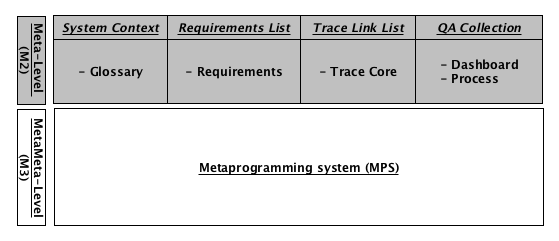
\includegraphics[width=1\textwidth]{./figures/Fig1.png}
\caption{A customizable language stack for gathering software requirements}
\label{fig:meta_struct_reqs}
\end{figure*}

\subsection{Customising the Requirements Gathering Framework: An Industrial Case
Study}
\label{sec:custom_frame}

Nowadays, many embedded hardware systems (e.g. in laptops, cars or
planes) are assembled together with cooling systems. The main purpose of
those cooling systems is to maintain an appropriate temperature during the
operation of those hardware electronics.

In this section we will extend the generic requirements gathering framework that
has been introduced in section~\ref{sec:generic_req_fram} in order to specialize it for
gathering requirements for software controllers for hardware cooling systems. In
particular, we will add a process for specifying this type of requirements. 

The case study we present here is inspired by a requirements document (that for
non-disclosure reasons we cannot cite here) that was made available to us by
Diehl aerospace, one of our industrial partners. Diehl builds hardware for
airplanes and, as such, cooling systems for that hardware also need to be
produced. The process of gathering requirements the software that controls such
cooling systems is currently almost completely manually done. This poses a
problem to Diehl, as the current requirements gathering process imposes a large
amount of effort to ensure that those requirements are documented in a fashion
that is complete, correct and traceable. Additionally, the aerospace industry
has to adhere to strict regulations such that their systems can be certified to
be used in production. Software reviewers require precise documentation for
requirements, which is difficult to produce and maintain when little automation
is available.

The work presented in this section constitutes our effort to provide
a proof-of-concept model-based development environment to the Diehl engineers
for the construction of requirements for hardware cooling systems.
Note that, although this customization work has been done at fortiss, the idea
is that in the future this work would be performed by a \emph{domain specific tool
developer} at Diehl. In a similar fashion, frameworks for gathering requirements for purposes
other than for cooling systems could also be customized using as basis the same
original set of languages as the one described in
section~\ref{sec:generic_req_fram}.

% The automation we present here is modelled as a set of tool-guided refinement
% steps, starting from abstract requirements and incrementally proceeding towards increasingly concrete ones. The idea behind the
% framework is that each refinement step will be done using an MPS language at the
% right level of abstraction. Constraints enforced by the such languages, together
% with analyses running on the background sheduled by a flow model will make sure
% that requirements are, to a large extent, well-formed by construction.\\

In order to specialize the language stack presented in
figure~\ref{fig:meta_struct_reqs} we have added the following languages:

% The framework languages that are utilized are as follows,
% \begin{itemize}
%   \item A Glossary language to define the domain specific glossary terms (e.g.,
%   min/max temprature values).
%   \item The Requirements language for constructing the requirement (e.g.,
%   requirment for the cooling system) 
%     \end{itemize}

\begin{itemize}
  \item The \textsf{Table} language, for defining the behavior of the
  controller for the cooling system.
  \item The \textsf{ModelProperty} Language, which contains algorithms
  implementing analyses of properties that are specific to the cooling system requirements gathering system.
\end{itemize}

Additionally, the \emph{domain specific tool developer} also builds a process
that will configure the dashboard's behavior. The dashboard assists the requirements engineer during
the construction of the requirements by displaying hints and press-button
actions that guide the refinement of the requirements model.

The dashboard is configured by a description of which hints should be
provided to the requirements engineer under which conditions. This information
is provided as an instance of the \textsf{Process} language.
In figure~\ref{fig:flow_statechart} we provide an example of such a process,
depicted as a statechart, for the	cooling controller requirements.  
The top part of each state in the figure includes the conditions that need to be satisfied such that the hint in the lower part of
that state is displayed on the dashboard. 

The conditions described on the statecharts' states are boolean properties that
are checked on the current state of the requirements project. These boolean
properties are implemented in the \textsf{ModelProperty} Language in
figure~\ref{fig:model_reqs}. This language is dedicated to holding the
algorithms that run the analyses required for our specific requirements
gathering system.

% Given they are
% specific to the cooling system requirements gathering framework, they are are
% defined at the model level of abstraction (M2), on top of the bare-bones
% requirements gathering framework.\levi{review levels of abstraction}

Hints can be of two types: \emph{creational} or \emph{informational}.
Creational hints enable the user to automatically generate new instances of
languages in order to complete the model. On the other hand, informational hints
serve as guidance steps to the user but are not associated with automatic
actions. This means the requirements engineer has to manually perform a set of
actions in order to further refine the requirements model and reach the next
state of refinement of the requirements model as defined in the hint model in
figure~\ref{fig:flow_statechart}. 

% Note that, when the hint is creational, the concepts that need to be created
% can also be declared together with any data that need to copied from the
% unrefined onto the refined model.

% The current dashboard allows the requirements engineer to perform a certain kind
% of analysis during the requirement construction. The analysis is implemented
% using the constraints.
% At present, the constraints are implemented for the individual models
% (requirement and table languages).

% The types of constraints implemented for performing the analysis are, 1) model
% properties constraints, 2) type-system constraints and 3) self-defined
% constraints.
% Examples of the analysis performed during the requirement construction is as
% follows,
% \begin{itemize}
%   \item If the Requirements model is empty or not
%   \item If the Glossary terms are defined in the requirements
%   \item If the values of the glossary terms (i.e., min/max) are set in the
%   Glossary model
%   \item If the parts of the Requirement model are completely defined or not
%   \item If the cooling function increasing/decreasing intervals are continuous
%   \item If the values of increasing and decreasing intervals are between the
%   preset min and max thresholds
% \end{itemize}


% During the requirement construction process the requirements engineer is guided
% by a set of hints. The implemented hints can be categorized as follows, 1) the creational hints and 2) the informational hints.
% Creational hints enables the user to perform actions automatically (e.g.,
% creating a new language instance) to complete the model. Whereas, the informational hint only
% serves as a guidance step to the user that is not associated with any
% action to be executed automatically. When an informational hint is provided to
% the user in the dashboard, the user has to manually perform the action in order
% to complete the requirement and resolve any errors. These errors in the
% requirement are caused because of the failed constraints
% discussed earlier.\saad{drafted}

\begin{figure*}[!h]
\centering
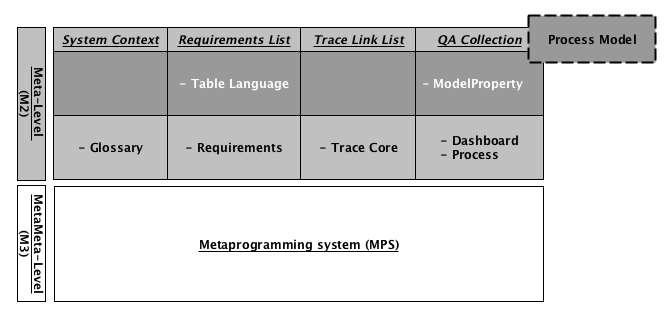
\includegraphics[width=1\textwidth]{./figures/Fig2.png}
\caption{A specialized language stack for gathering software requirements
}
\label{fig:model_reqs}
\end{figure*}

For clarity reasons, let us now briefly explain the process model depicted in
figure~\ref{fig:flow_statechart}. The requirements engineer is initially
provided with an empty dashboard with a creational hint to start constructing
the requirements for the cooling controller.
At this point an empty requirements project can be automatically built using the
creational hint. An informational hint is then provided to guide the
requirements engineer through defining the threshold values as glossary terms in
the requirement and/or complete the requirements with all necessary data.
Upon successfully building a requirement and defining the glossary terms, the
requirements engineer is provided with a creational hint to perform the
refinement step from a requirement and its threshold values into a cooling
function describing the behavior of the controller.
An empty cooling function (i.e., a model of the \textsf{Table} language) is then
automatically created with the minimum and maximum thresholds values coming from
the glossary terms. The user is then provided with feedback from the
\textsf{Table} language until a correct cooling function is defined.

% at which
% point the user is provided with an informational hint that this part of the
% requirements is finished.

\begin{figure*}[!h]
\centering
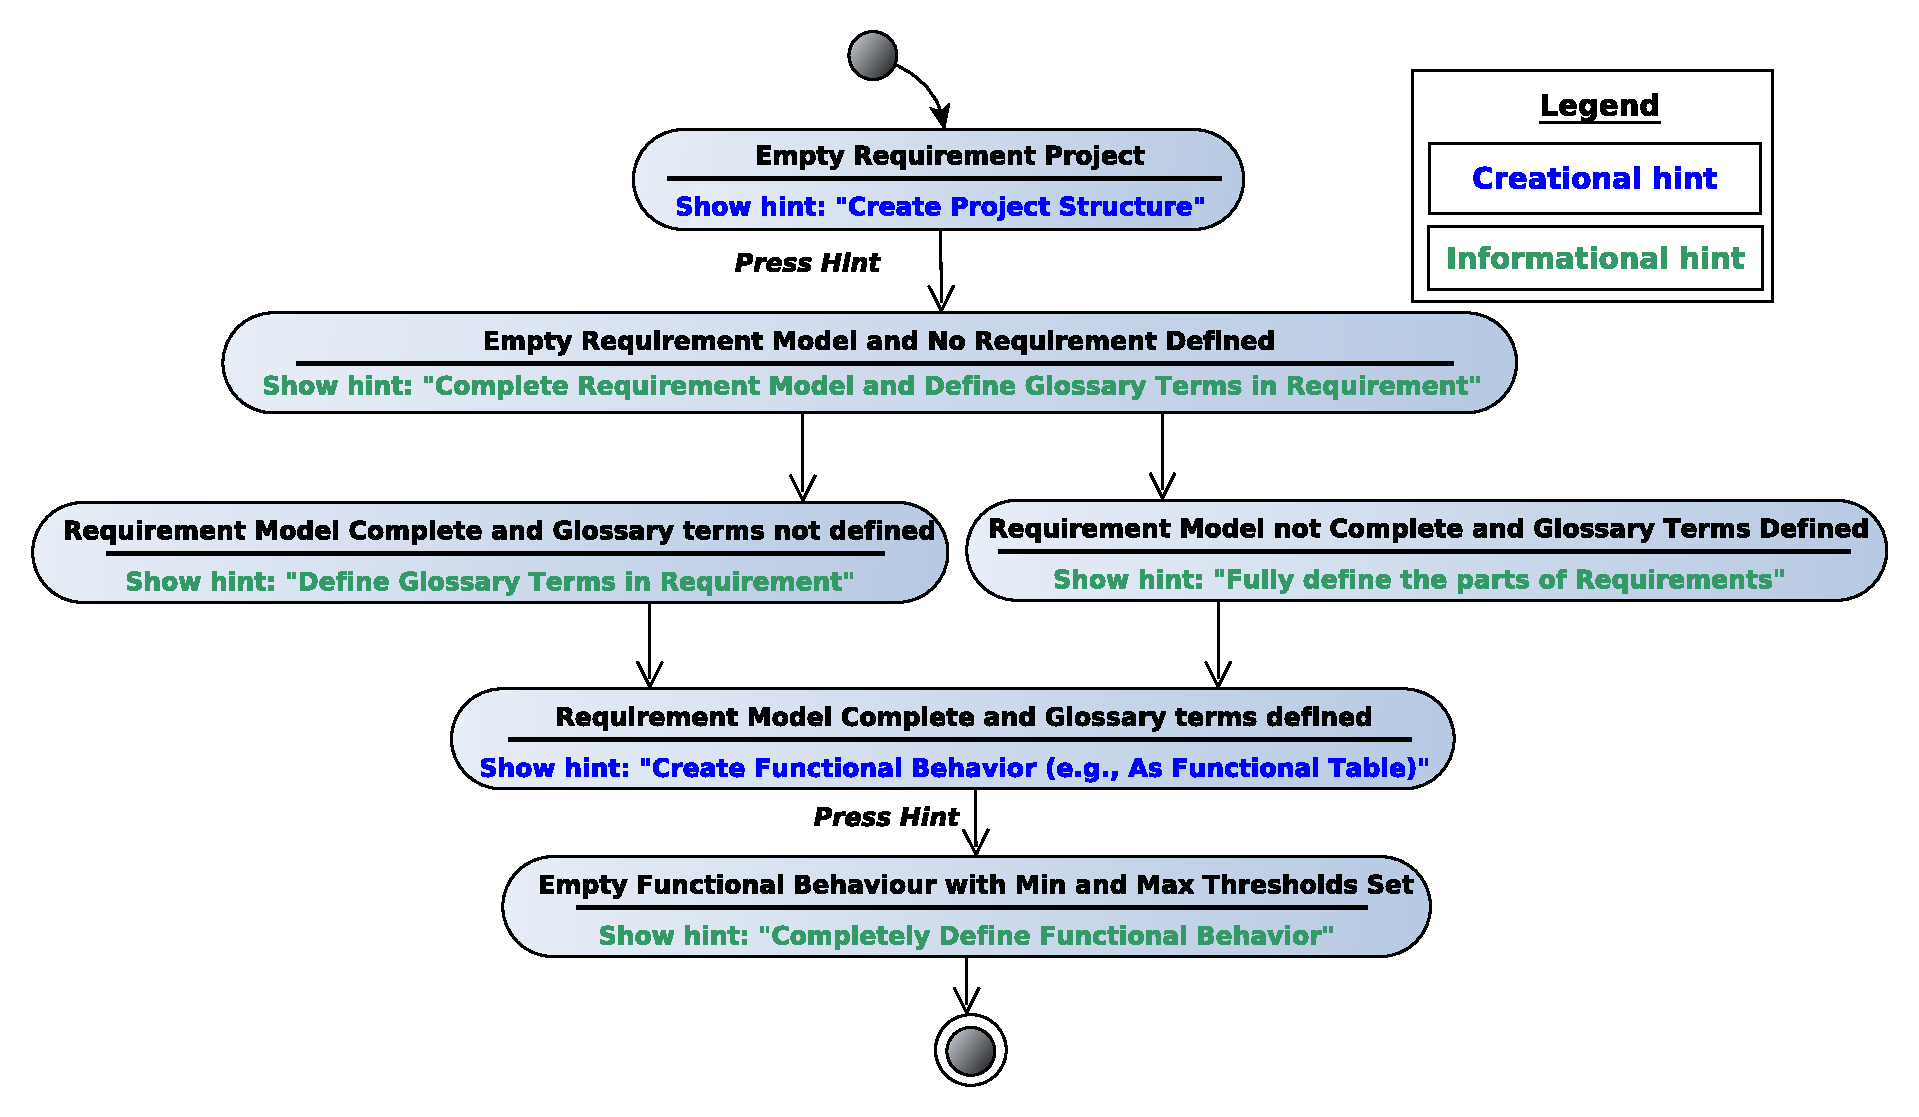
\includegraphics[width=1\textwidth]{./figures/FlowChart_V2.pdf}
\caption{A statechart-like representation of an instance of the \textsf{Flow}
language}
\label{fig:flow_statechart}
\end{figure*}

% Note that the \emph{flow} language example in figure~\ref{fig:flow_statechart} is
% only an example of a possible flow. Arbitrary flows for describing any
% requirements gathering framework can be defined, built on top of also arbitrary
% boolean property checks defined in the \emph{custom analysis} language.

% There exits some limitations in the current implementation of the
% dashboard that are as follows,
% \begin{itemize}
%   \item for now the dashboard content and the hints are hardcoded in the
%   dashboard language
%   \item the dashboard should be an independent language, to be extended with
%   the holding specific models in the particular project.
%    \item a hint language for the flow can be defined as a statechart. Such
%    models would then need to be compiled (using an intention) to produce the
%    necessary transform actions in the dashboard language. The Dashboard language
%    should then be recompiled after the intention to generate the transform
%    actions is ran.
%    \item In the current version of the dashboard there are boolean constraints implemented. An example
% of a boolean constraint is to check if a particular property of a model is set
% or not (e.g., type of a requirement is set or not). At present we require more
% complex checking
%   \item Constraints are defined as methods in a separate language over the
%   languages on top of which the analysis should be defined.\saad{limitations
%   are our next steps. can be put in the future work section of the paper}
%       \end{itemize}

% MIRA aims at improving the quality of system under development by
% supporting quality assurance (QA).  At this level we had to extend the existing MPS framework with languages
% to define \emph{flow} and a \emph{dashboard} (although hard-code extensions would
% be the way to go for the future).
% 
% % The MIRA framework has been implemented as a
% % requirement specification plugin for the Autofocus environment~\cite{AF315}. In
% % particular, under the AF3 environment the MIRA framework provides an integrated
% % envrionment for building and formalizing the requirements for a particular
% % system under development.
% 
% At the meta level the framework to build the composed models for requirements is
% assembled. This framework consists of:
% 
% \begin{itemize}
%   \item A set of brick languages defined using MPS' metametalevel.
%   \item A set of constraints that extend the extension points defined at the
%   metametalevel.
%   \item A set of action hints associated to the constraints.
%   \item Levels of priority of satisfaction of constraints. A level includes a
%   set of constraints and a level is accomplished when all the constraints are
%   satisfied. Satisfying a sequence of levels will lead to the desired
%   composed model (analogy with gamification). Special attention has to be paid
%   to when checks have been satisfied but then stop being so. A statemachine
%   associated to the levels of priority should be kept updated as the composed
%   model gets updated by the user.
% \end{itemize}
% 
% 
% Our tool/dashboard is a guiding system that uses the
% requirements model along with some glossary terms (e.g., min/max values for the
% cooling system) for requirement construction. It also enables the user to
% perform refinements of the constructed requirement into an expected behavioral function (e.g., cooling
% function in our case study). These refinements are configured as a flow model
% implemented by a set of hints that are associated with the constraints.
% The flow model is implemented through a set of hints in our built
% tool/dashboard. \saad{text moved from model level}
% Additionally, we have provided extension points to give the user the possibility to define her own constraints
% that can be used to direct the flow of edition of the composed model.
% 
% \begin{itemize}
%   \item the Diehl case study
%   \item composing languages through traceability (and just MPS inclusion)
%   \item following Sabine's notion of requirements quality and instantiating MIRA
%   (using domain-level (inter-language) checks)
%   \item define a completion dashboard to guide the user through
%   formalizing requirements
% \end{itemize}

% \begin{figure*}[!h]
% \centering
% 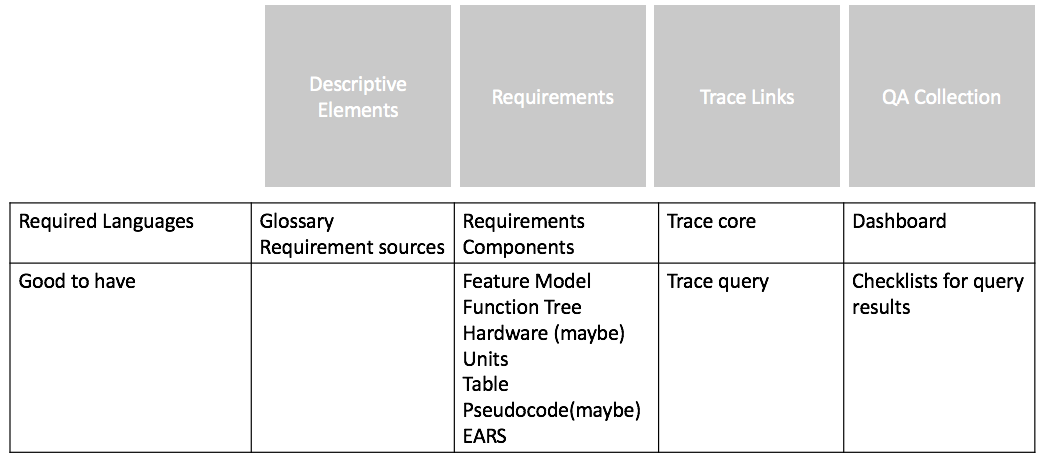
\includegraphics[width=\textwidth]{./figures/core_languages.png}
% \caption{Meta-structure for the definition of requirements gathering
% frameworks}
% \label{fig:meta_struct_reqs}
% \end{figure*}